\section{Games as a Recursive Data Type}

Chess, Checkers, and Tic-Tac-Toe are examples of \emph{two-person
terminating games of perfect information}, ---$\tg$'s for short.  These
are games in which two players alternate moves that depend only on the
visible board position or state of the game.  ``Perfect information''
means that the players know the complete state of the game at each move.
(Most card games are \emph{not} games of perfect information because
neither player can see the other's hand.)  ``Terminating'' means that play
cannot go on forever ---it must end after a finite number of
moves.\footnote{Since board positions can repeat in chess and checkers,
termination is enforced by rules that prevent any position from being
repeated more than a fixed number of times.  So the ``state'' of these
games is the board position \emph{plus} a record of how many times
positions have been reached.}

We will define $\tg$'s \iffalse in a straightforward way tagged\fi as a 
recursive data type.  To see how this will work, let's use the game of
Tic-Tac-Toe as an example.

\subsection{Tic-Tac-Toe}

Tic-Tac-Toe is a game for young children.  There are two players who
alternately write the letters ``X'' and ``O'' in the empty boxes of a $3
\times 3$ grid.  Three copies of the same letter filling a row, column, or
diagonal of the grid is called a \emph{tic-tac-toe}, and the first player
who gets a tic-tac-toe of their letter wins the game.  \iffalse Children
generally don't take long to figure out an optimal strategy for playing the
game.\fi


We're now going give a precise mathematical definition of the Tic-Tac-Toe
\term{game tree} as a recursive data type.  \iffalse and carefully defining
the allowed moves Children of course have no need for such a definition,
and it would be too complicated for them anyway.  But if we had to write a
Tic-Tac-Toe playing \emph{computer program}, we'd need this kind of picky
precision.\fi Here's the idea behind the definition: at any point in the
game, the ``board position'' is the pattern of X's and O's on the $3 \times
3$ grid.  From any such Tic-Tac-Toe pattern, there are a number of next
patterns that might result from a move.  For example, from the initial
empty grid, there are nine possible next patterns, each with a single X in
some grid cell and the other eight cells empty.  From any of these
patterns, there are eight possible next patterns gotten by placing an O in
an empty cell.  These move possibilities are given by the
\hyperdef{game}{tree}{game tree} for Tic-Tac-Toe indicated in
Figure~\ref{fig:Tic-Tac-Toe}.

\begin{figure}[htbp]
\centering
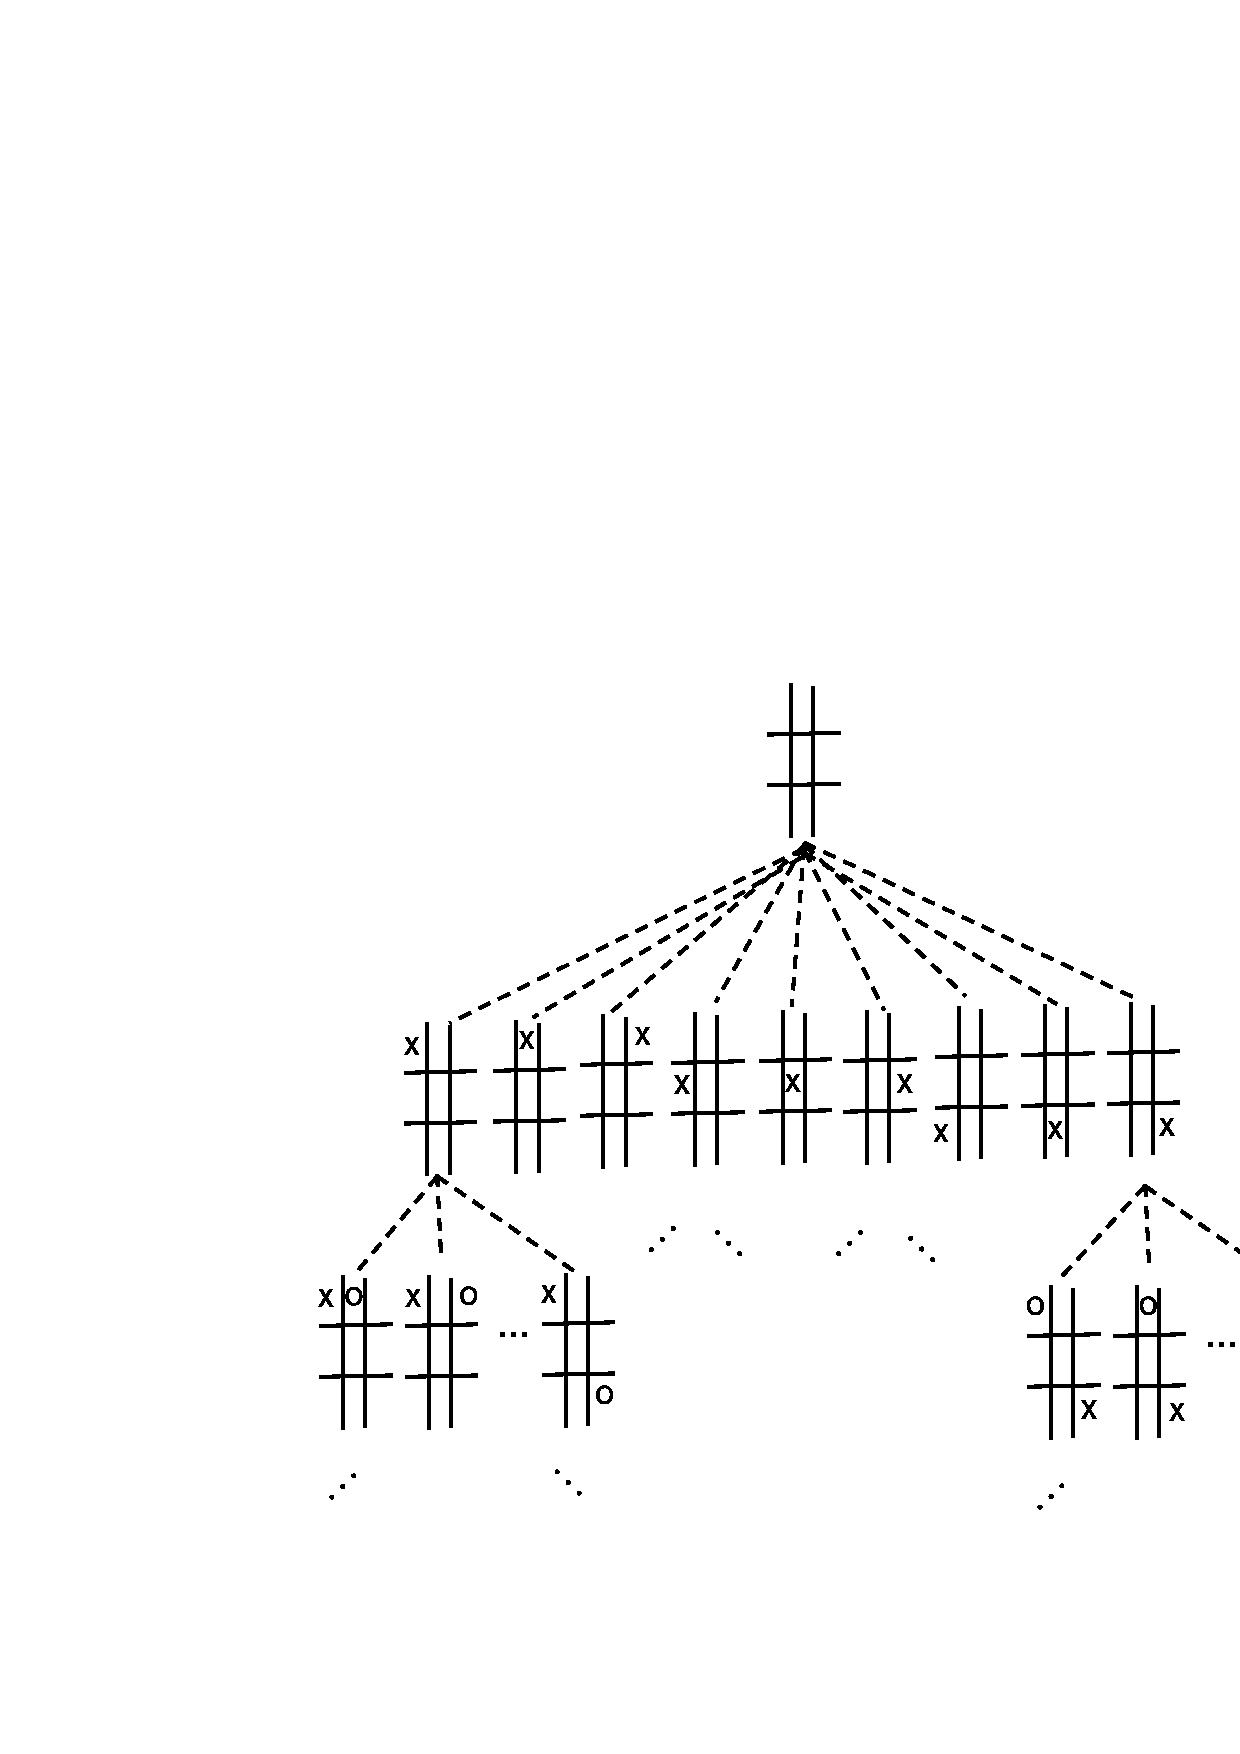
\includegraphics[height=6in]{figures/topgame.pdf}
\caption{The Top of the Game Tree for Tic-Tac-Toe.}
\label{fig:Tic-Tac-Toe}
\end{figure}


\iffalse
\[\begin{array}{c|c|c}
\hspace{.1in} & \hspace{.1in} & \hspace{.1in}\\
\hline  & &\\
\hline  & &
\end{array}\]

\textbf{FIGURE NEEDED}
\fi

\begin{definition}

A Tic-Tac-Toe \emph{pattern} is a $3 \times 3$ grid each of whose 9 cells
contains either the single letter, X, the single letter, O, or is
empty.
\iffalse
Moreover, there must be either
\begin{itemize}

\item one more X than O's, with at most two tic-tac-toes of X's, and no
tic-tac-toe of O's, or

\item an equal number of X's and O's, with at most one tic-tac-toes of
O's, and no tic-tac-toe of X's.
\end{itemize}
\fi

A pattern, $Q$, is a \emph{possible next pattern after} $P$, providing $P$
has no tic-tac-toes and
\begin{itemize}

\item if $P$ has an equal number of X's and O's, and $Q$ is the same as
$P$ except that a cell that was empty in $P$ has an X in $Q$, or

\item if $P$ has one more X than O's, and $Q$ is the same as $P$ except
that a cell that was empty in $P$ has an O in $Q$.
\end{itemize}

If $P$ is a Tic-Tac-Toe pattern, and $P$ has no next patterns, then the
\emph{terminated Tic-Tac-Toe game trees} at $P$ are

\begin{itemize}

\item 
\[
\ang{P, \ang{\texttt{win}}},
\]
if $P$ has a tic-tac-toe of X's.


\item 
\[
\ang{P, \ang{\texttt{lose}}},
\]
if $P$ has a tic-tac-toe of O's.


\item
\[
\ang{P, \ang{\texttt{tie}}},
\]
otherwise.

\end{itemize}


\iffalse
If $Q$ is a possible move from $P$, then the game tree starting at $Q$ is
called a \emph{  Notice
that $\mathcal{G}_P = \emptyset$ iff $P$ is terminated.}
\fi

The \emph{Tic-Tac-Toe game trees starting at $P$} are defined recursively:

\textbf{Base Case}:
A terminated Tic-Tac-Toe game tree at $P$ is a Tic-Tac-Toe game tree
starting at $P$.

\textbf{Constructor case}: If $P$ is a non-terminated Tic-Tac-Toe pattern,
then the Tic-Tac-Toe game tree starting at $P$ consists of $P$ and the set
of all games trees starting at possible next patterns after $P$.
\end{definition}

For example, if
\begin{align*}
P_0 & =  \begin{array}{c|c|c}
                O & X & O\\
         \hline X & O & X\\
         \hline X & &
        \end{array}\\
Q_1 & = \begin{array}{c|c|c}
                O & X & O\\
         \hline X & O & X\\
         \hline X &  & O
        \end{array}\\
Q_2 & = \begin{array}{c|c|c}
                O & X & O\\
         \hline X & O & X\\
         \hline X & O & 
        \end{array}\\
R & = \begin{array}{c|c|c}
                O & X & O\\
         \hline X & O & X\\
         \hline X & O & X
        \end{array}
\end{align*}
the game tree starting at $P_0$ is pictured in Figure~\ref{fig:endgame}.

\iffalse
Then,
\begin{equation}\label{endgame}
\ang{P, \set{\ang{Q_1, \ang{\texttt{lose}}},
             \ang{Q_2, \set{\ang{R,\ang{\texttt{tie}}}}}}}
\end{equation}
is the tagged recursive datum that corresponds to a Tic-Tac-Toe ``end
game'' that starts with $P$.  This game is easier to understand by looking
at its game tree in Figure~\ref{fig:endgame}.  Notice that the game tree
---which so far we haven't actually defined ---is simply the parse tree of
the tagged datum.\fi


\begin{figure}[htbp]
\centering
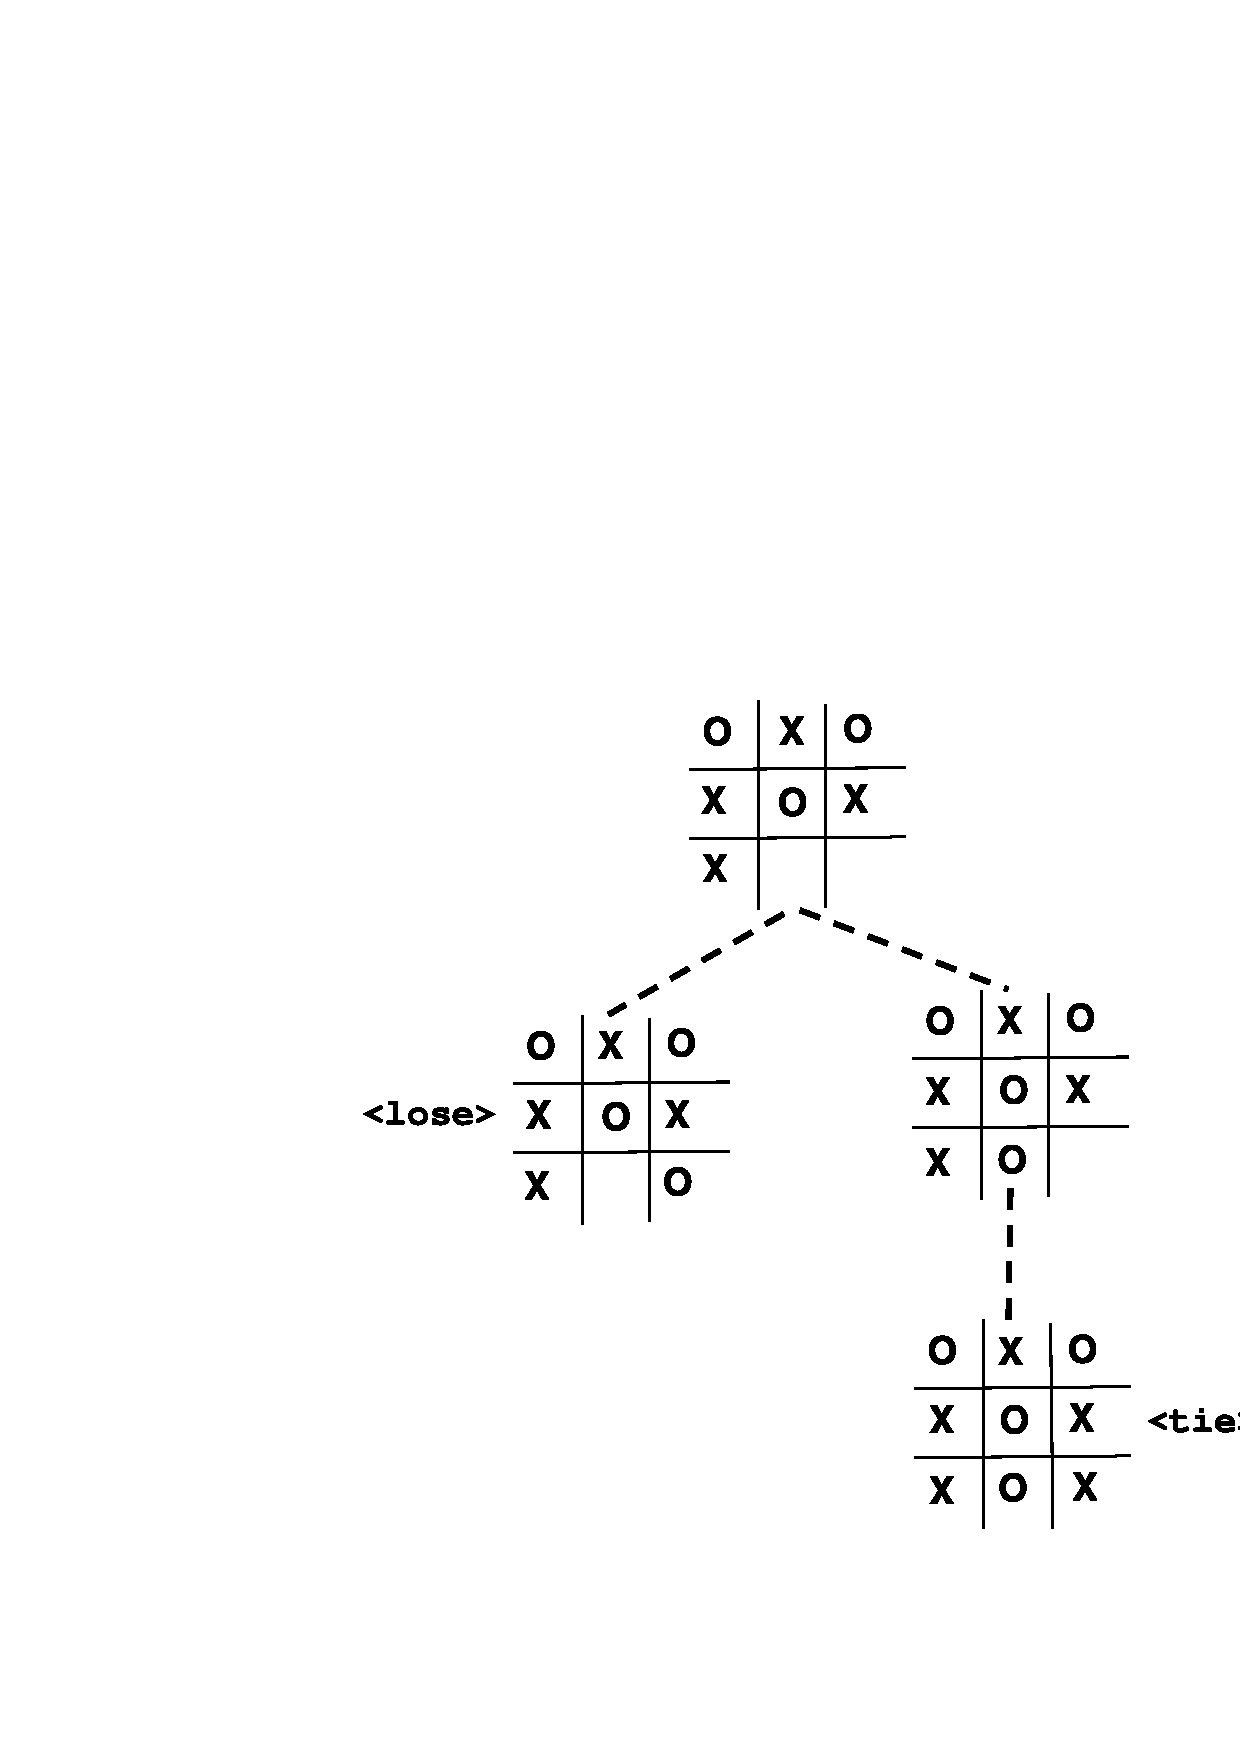
\includegraphics[height=4in]{figures/endgame.pdf}
\caption{Game Tree for the Tic-Tac-Toe game starting at $P_0$.}
\label{fig:endgame}
\end{figure}

Game trees are usually pictured in this way with the starting pattern
(referred to as the ``root'' of the tree) at the top and lines connecting
the root to the \iffalse roots of the \fi game trees that start at each
possible next pattern.  The ``leaves'' at the bottom of the tree (trees
grow upside down in Computer Science) correspond to terminated games.  A
path from the root to a leaf describes a complete \emph{play} of the game.
(In English, ``game'' can be used in two senses: first we can say that
Chess is a game, and second we can play a game of Chess.  The first usage
refers to the data type of Chess game trees, and the second usage refers to
a ``play.'')

\subsection{Infinite Tic-Tac-Toe Games}

At any point in a Tic-Tac-Toe game, there are at most nine possible next
patterns, and no play can continue for more than nine moves.  But suppose
we consider an \emph{$n$-game Tic-Tac-Toe tournament} where the tournament
winner is the one who wins more of $n>0$ individual Tic-Tac-Toe games.  (If
they each win an equal number of individual games, then the tournament is a
tie.)

Now we can consolidate all these tournaments into a single game we can call
\emph{Tournament-Tic-Tac-Toe}: the first player in Tournament-Tic-Tac-Toe
chooses any integer $n > 0$, and then the players play an $n$-game
tournament.  Now there are infinitely many possible first moves: the first
player can choose $n=1$, or $n=2$, or $n=3$, or \dots.  But still, it's
obvious that every possible play of Tournament-Tic-Tac-Toe is finite,
because after the first player chooses a value for $n$, the game can't
continue for more than $9n$ moves.  So it's not possible to keep playing
forever even though the game tree is infinite.

This isn't very hard to understand, but there is an important difference
between any given $n$-game tournament and Tournament-Tic-Tac-Toe: even
though every play of Tournament-Tic-Tac-Toe must come to an end, there is
no longer any bound on how many moves it might be before the game ends ---a
play might end after 9 moves, or $9(2001)$ moves, or $9(10^{10}+1)$ moves;
it just can't continue forever.

\iffalse While there is no bound on how long to play, at least after the
first move to an $n \times n$ board in meta-Tic-Tac-Toe, we know the game
will end with $n^2$ moves.\fi

With Tournament-Tic-Tac-Toe recognized as a \tg, we can go on to
Tournament$^2$-Tic-Tac-Toe where the first player chooses a number, $m>0$,
of Tournament-Tic-Tac-Toe games to play, and the second player acts as the
first player in each of the $m$ Tournament-Tic-Tac-Toe games to be played.
Then, of course, there's Tournament$^3$-Tic-Tac-Toe\dots.

\iffalse Every play of the meta-meta game must still end, but now even
after the first move, there is no bound on how long a game might
continue.\fi

\subsection{Two Person Terminating Games}

Familiar games like Tic-Tac-Toe, Checkers, and Chess can all end in ties,
but for simplicity we'll only consider win/lose games ---no ``everybody
wins''-type games at MIT. \texttt{:-)}.  But everything we show about
win/lose games will extend easily to games with ties.

\iffalse
Of course Tic-Tac-Toe and the
other games will fit this set up if we treat a game that ends in a tie as
a loss for the usual first player ---White in Chess, Red in Checkers, the
X-player in Tic-Tac-Toe.
\fi

Like Tic-Tac-Toe, the idea behind the definition of $\tg$'s as a recursive
data type is that making a move in a $\tg$ leads to the start of a subgame.
For Tic-Tac-Toe, we used the patterns and the rules of Tic-Tac-Toe to
determine the next patterns.  But once we have a complete game tree, we
don't really need the pattern labels: the root of a game tree itself can
play the role of a ``board position'' with its possible ``next positions''
determined by the roots of its subtrees.  This leads to the following very
simple ---perhaps deceptively simple ---general definition.

\begin{definition}
The \hyperdef{2p}{tg}{$\tg$}, \emph{game trees for two-person terminating
    games of perfect information} are defined recursively as follows:
\begin{itemize}

\item \textbf{Base cases:}
\[\begin{array}{ll}
\ang{\texttt{leaf},\texttt{win}} & \in \tg, \text{ and}\\
\ang{\texttt{leaf},\texttt{lose}}& \in \tg.
\end{array}\]

\item \textbf{Constructor case:}
If $\mathcal{G}$ is a nonempty set of
$\tg$'s, then $G$ is a $\tg$, where
\[
G \eqdef \ang{\texttt{tree},\mathcal{G}}.
\]
The games trees in $\mathcal{G}$ are called the possible \emph{next moves}
from $G$.
\end{itemize}

\end{definition}

These games are called ``terminating'' because, even though a $\tg$ may be
a (very) infinite datum like Tournament$^2$-Tic-Tac-Toe, every play of a
$\tg$ must terminate.  This is something we can now prove, after we give a
precise definition of ``play'':

\begin{definition}
A \emph{play} of a $\tg$, $G$, is a (potentially infinite) sequence of
$\tg$'s starting with $G$ and such that if $G_1$ and $G_2$ are consecutive
$\tg$'s in the play, then $G_2$ is a possible next move of $G_1$.

If a $\tg$ has no infinite play, it is called a \emph{terminating} game.
\end{definition}

\begin{theorem}
Every $\tg$ is terminating.
\end{theorem}

\begin{proof}
By structural induction on the definition of a $\tg$, $G$, with induction
hypothesis
\[
G \text{ is terminating}.
\]

\textbf{Base case}: If $G = \ang{\texttt{leaf}, \texttt{win}}$ or $G =
\ang{\texttt{leaf}, \texttt{lose}}$ then the only possible play of $G$ is
the length one sequence consisting of $G$.  Hence $G$ terminates.

\textbf{Constructor case}: For $G = \ang{\texttt{tree},\mathcal{G}}$, we
must show that $G$ is terminating, given the Induction Hypothesis that
\emph{every} $G' \in \mathcal{G}$ is terminating.

But any play of $G$ is, by definition, a sequence starting with $G$ and
followed by a play starting with some $G_0 \in \mathcal{G}$.  But $G_0$ is
terminating, so the play starting at $G_0$ is finite, and hence so is the
play starting at $G$.

This completes the structural induction, proving that every \tg, $G$, is
terminating.
\end{proof}


\subsection{Game Strategies}

A key question about a game is whether a player has a winning strategy.  A
\emph{strategy} for a player in a game specifies which move the player
should make at any point in the game.  A \emph{winning} strategy ensures
that the player will win no matter what moves the other player makes.

In Tic-Tac-Toe for example, most elementary school children figure out
strategies for both players that each ensure that the game ends with no
tic-tac-toes, that is, it ends in a tie.  Of course the first player can
win if his opponent plays childishly, but not if the second player follows
the proper strategy.  In more complicated games like Checkers or Chess,
it's not immediately clear that anyone has a winning strategy, even if we
agreed to count ties as wins for the second player.

But structural induction makes it easy to prove that in any $\tg$,
\emph{somebody} has the winning strategy!

\begin{theorem}\label{fund}
\textbf{Fundamental Theorem for Two-Person Games:} For every two-person
terminating game of perfect information, there is a winning strategy for
one of the players.
\end{theorem}

\begin{proof}
The proof is by structural induction on the definition of a $\tg$, $G$.
The induction hypothesis is that there is a winning strategy for $G$.

\textbf{Base cases:}
\begin{enumerate}

\item $G=\ang{\texttt{leaf}, \texttt{win}}$.  Then the first player has the
 winning strategy: ``make the winning move.''

\item $G=\ang{\texttt{leaf}, \texttt{lose}}$.  Then the second player has a
 winning strategy: ``Let the first player make the losing move.''
\end{enumerate}

\textbf{Constructor case}: Suppose $G = \ang{\texttt{tree},\mathcal{G}}$.
By structural induction, we may assume that some player has a winning
strategy for each $G' \in \mathcal{G}$.  There are two cases to consider:
\begin{itemize}
\item some $G_0 \in \mathcal{G}$ has a winning strategy for its second
  player.  Then the first player in $G$ has a winning strategy: make the
  move to $G_0$ and then follow the second player's winning strategy in
  $G_0$.

\item every $G' \in \mathcal{G}$ has a winning strategy for its first
  player.  Then the second player in $G$ has a winning strategy: if the
  first player's move in $G$ is to $G_0 \in \mathcal{G}$, then follow the
  winning strategy for the first player in $G_0$.
\end{itemize}
So in any case, one of the players has a winning strategy for $G$, which
completes the proof of the constructor case.

It follows by structural induction that there is a winning strategy for
every $\tg$, $G$.
\end{proof}

Notice that although Theorem~\ref{fund} guarantees a winning strategy, its
proof gives no clue which player has it.  For
\iffalse the Subset Takeaway Game
(\href{http://courses.csail.mit.edu/6.042/fall07/rec3t.pdf} {Recitation
Problem, Tuesday, Week 3}), and
\fi
most familiar $\tg$'s like Checkers, Chess, Go, \dots, no one knows
which player has a winning strategy.

\endinput